% $Header$

\documentclass{beamer}
\usefonttheme[onlymath]{serif}
\newcommand\bmale{\fontsize{6}{7.2}\selectfont}
\newcommand\male{\fontsize{8}{7.2}\selectfont}
\newcommand\normalne{\fontsize{10}{7.2}\selectfont}
\newcommand\duze{\fontsize{12}{7.2}\selectfont}
\setbeamertemplate{caption}{\raggedright\insertcaption\par}
% This file is a solution template for:

% - Talk at a conference/colloquium.
% - Talk length is about 20min.
% - Style is ornate.



% Copyright 2004 by Till Tantau <tantau@users.sourceforge.net>.
%
% In principle, this file can be redistributed and/or modified under
% the terms of the GNU Public License, version 2.
%
% However, this file is supposed to be a template to be modified
% for your own needs. For this reason, if you use this file as a
% template and not specifically distribute it as part of a another
% package/program, I grant the extra permission to freely copy and
% modify this file as you see fit and even to delete this copyright
% notice. 


\mode<presentation>
{
  \usetheme{CambridgeUS}
  \usecolortheme{beaver}
  % or ...

  %\setbeamercovered{transparent}
  % or whatever (possibly just delete it)
}

\usepackage{ulem}
\usepackage{tabto}
\usepackage[]{algorithm2e}
\usepackage{bm}
\usepackage{lmodern}
\usepackage[T1]{fontenc}
\usepackage[polish]{babel}
\usepackage[utf8]{inputenc}
\DeclareMathOperator*{\argmin}{argmin}
\DeclareMathOperator*{\argmax}{argmax}
\selectlanguage{polish}
% or whatever

%\usepackage[latin1]{inputenc}
%% or whatever

% Or whatever. Note that the encoding and the font should match. If T1
% does not look nice, try deleting the line with the fontenc.


\title[Analizy mikrosymulacyjne] % (optional, use only with long paper titles)
{Analizy mikrosymulacyjne - wykłady}

\subtitle
{Model mikroskopowy I}

\author[dr inż. Rafał Kucharski] % (optional, use only with lots of authors)
{dr inż. Rafał~Kucharski\inst{1}}
% - Give the names in the same order as the appear in the paper.
% - Use the \inst{?} command only if the authors have different
%   affiliation.

\institute[] % (optional, but mostly needed)
{
  \inst{1}%
  Zakład Systemów Komunikacyjnych\\
  Politechnika Krakowska
  \and
 }
% - Use the \inst command only if there are several affiliations.
% - Keep it simple, no one is interested in your street address.

\date[ZSK, L-2, WIL, PK] % (optional, should be abbreviation of conference name)
{Kraków, 2017}
% - Either use conference name or its abbreviation.
% - Not really informative to the audience, more for people (including
%   yourself) who are reading the slides online



% If you have a file called "university-logo-filename.xxx", where xxx
% is a graphic format that can be processed by latex or pdflatex,
% resp., then you can add a logo as follows:

\pgfdeclareimage[height=1cm]{university-logo}{ZSK}
 \logo{\pgfuseimage{university-logo}}

% Delete this, if you do not want the table of contents to pop up at
% the beginning of each subsection:
\AtBeginSubsection[]
%{
%  \begin{frame}<beamer>{Outline}
%    \tableofcontents[currentsection,currentsubsection]
%  \end{frame}
%}


% If you wish to uncover everything in a step-wise fashion, uncomment
% the following command: 

%\beamerdefaultoverlayspecification{<+->}


\begin{document}

\begin{frame}
  \titlepage
\end{frame}

%\begin{frame}{Zakres}
%  \tableofcontents
%  % You might wish to add the option [pausesections]
%\end{frame}


% Structuring a talk is a difficult task and the following structure
% may not be suitable. Here are some rules that apply for this
% solution: 

% - Exactly two or three sections (other than the summary).
% - At *most* three subsections per section.
% - Talk about 30s to 2min per frame. So there should be between about
%   15 and 30 frames, all told.

% - A conference audience is likely to know very little of what you
%   are going to talk about. So *simplify*!
% - In a 20min talk, getting the main ideas across is hard
%   enough. Leave out details, even if it means being less precise than
%   you think necessary.
% - If you omit details that are vital to the proof/implementation,
%   just say so once. Everybody will be happy with that.
\section{Wykład 2: Model mikroskopowy I}
\subsection{Wstęp}

\begin{frame}{Wstęp}{miejsce symulacji w modelowaniu podróży i ruchu}
\begin{center}
Pełny rozkład ruchu na sieć (ostatni krok modelu czterostadiowego)
\\ np. metoda równowagi \alert{Wardop'a} \\
\includegraphics[scale=0.4]{assign}
\end{center}
\end{frame}

\begin{frame}{Wstęp}{miejsce symulacji w modelowaniu podróży i ruchu}
\begin{center}
\includegraphics[scale=0.2]{assign}
\end{center}
\male
W tej pętli iteracyjnej:
\begin{itemize}
\item  górna część to wybór ścieżki \textit{route-choice model}, 
\item dolna to model funkcjonowania sieci (\textit{network performance model}), w zależności od modelu:
\begin{itemize}
\male
\item makroskopowy statyczny (Visum i funkcja oporu)
\item makroskopowy dynamiczny (PTV Optima i diagram fundamentalny)
\item symulacja mikroskopowa (PTV Vissim i model Wiedemanna)
\item model wieloagentowy (MATSim i automaty komórkowe)
\item jakikolwiek inny model który określa koszty (czas, długośc kolejki, i in.) dla zadanego popytu (obciążenia ścieżek).
\end{itemize}
\end{itemize}
\end{frame}

\begin{frame}{Wstęp}{rola symulacji mikroskopowej}
\alert{Symulacja mikroskopowa}\\
\textbf{dla zadanego popytu} $Q_k(t)$ - obciążenie ścieżek $k$ \textbf{określ  koszty przejazdu pojazdów zadanymi ścieżkami}\\ ~\\
\par
\alert{Rozkład ruchu na sieć}\\
\textbf{dla zadanego popytu} $Q_{od}(t)$ - więźba \textbf{określ ścieżki generujące koszty spełniające warunki równowagi Wardop'a}\\ 
\begin{equation}
q_k \cdot  \left( c_k - \tilde{c}_{od}) \right) = 0
\end{equation}
\begin{equation*}
\tilde{c}_{od} = min_{k \in K_{od}} (c_k)
\end{equation*}
\begin{equation}
\sum_{k \in K_{od}} q_k = q_{od}
\end{equation}
\end{frame}

\begin{frame}{Wstęp}{rola symulacji mikroskopowej}
Znacznie mniej niż rozkład ruchu \\
\begin{enumerate}
\item ścieżki (trasy przejazdu) są stałe
\item brak wpływu zatłoczenia na zmianę trasy
\item jak obliczane są trasy przejazdu? 
\item jak zmiana w organizacji wpłynie na zmianę ścieżek?
\end{enumerate}
\begin{center}
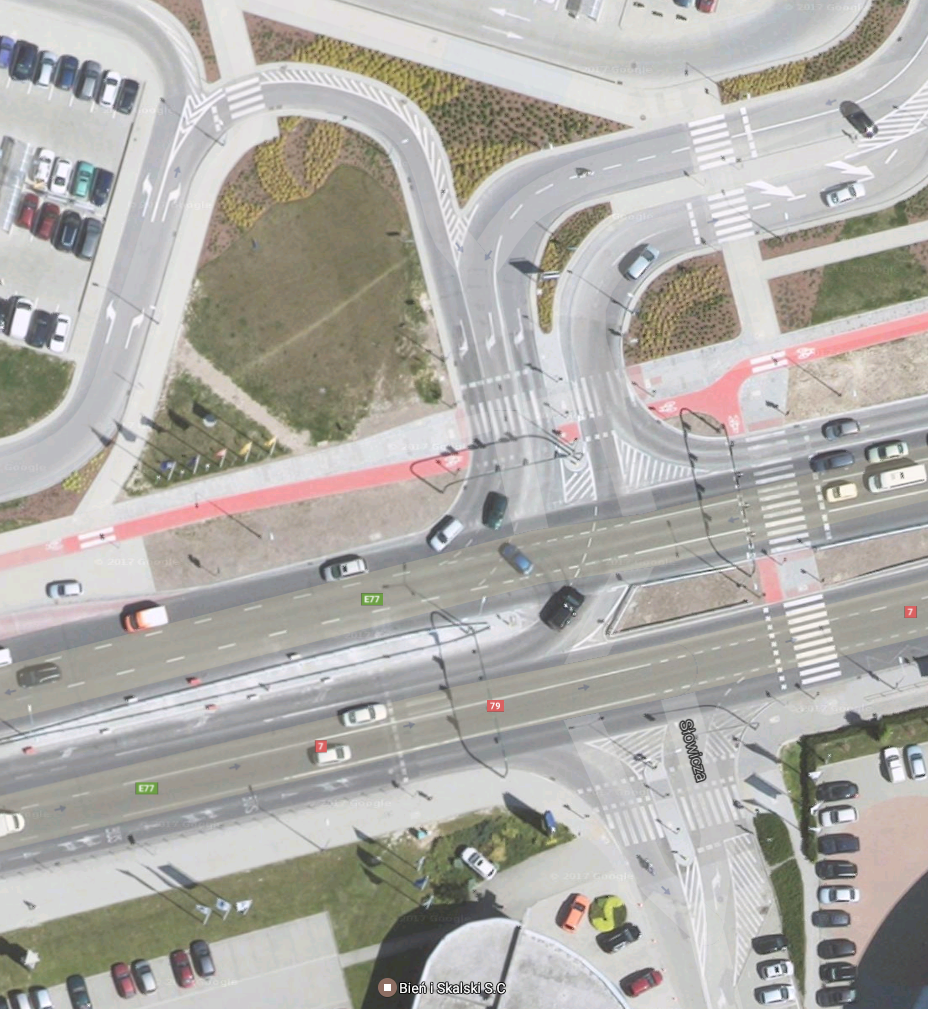
\includegraphics[scale=0.15]{ikea}
\end{center}
\end{frame}


\begin{frame}{Wstęp}{symulacja mikroskopowa}
Mikrosymulacja ruchu: 
\begin{itemize}
\item każdy \textbf{obiekt} (pojazd $\alpha$) w \textbf{układzie} (sieć drogowa wraz z pojazdami) \\
\item w każdej chwili czasu ($t \in T$)
\item podejmuje \textbf{decyzje} (o przyśpieszeniu, włączeniu się do ruchu, zmianie pasa, skręcie, $\dots$)
\begin{itemize}
\item subiektywnie \textbf{optymalne} (dotrzeć do celu minimalnym kosztem)
\item na podstawie \textbf{opisu stanu} (położenie i kierunek mój i innych obiektów w układzie)
\end{itemize}
\end{itemize}
\end{frame}

\subsection{Graf}
\begin{frame}{Graf}{reprezentacja sieci drogowej}\end{frame}

\begin{frame}{Graf mikroskopowy}{reprezentacja sieci}
\begin{columns}
\column{0.4\textwidth}
 \includegraphics[scale=0.4]{vissimnet}
\column{0.6\textwidth}
 \male
  \begin{itemize}
  \item graf $G(N,A)$, ale dualny, kluczową rolę pełnią relacje skrętne (połączenia między odcinkami)
  \item odcinki $a$ to jednorodne przekroje pomiędzy miejscami zmiany geometrii
  \item węzły $n$ to punkty zmian w geometrii (włączenia, przecięcia, rozjazdy, itp.)
  \item relacje skrętne $t$ to możliwości kontynuacji jazdy pomiędzy odcinkami
  \end{itemize}
  wobec tego \textbf{położenie} $x_\alpha$ pojazdu jest określone poprzez element grafu na którym znajduje się pojazd w danym czasie, oraz:
   \begin{itemize}
   \item podłużnie  $x_\alpha(t) \in R^+$ (rośnie od początku odcinka do końca)
   \item poprzeczne $n_\alpha(t) \in N$(pas).
   \end{itemize}
\end{columns}
\end{frame}

\begin{frame}{Graf mikroskopowy}{graf dualny}

\begin{center}
$G(N,A) \rightarrow G(A,T)$ \\~\\
 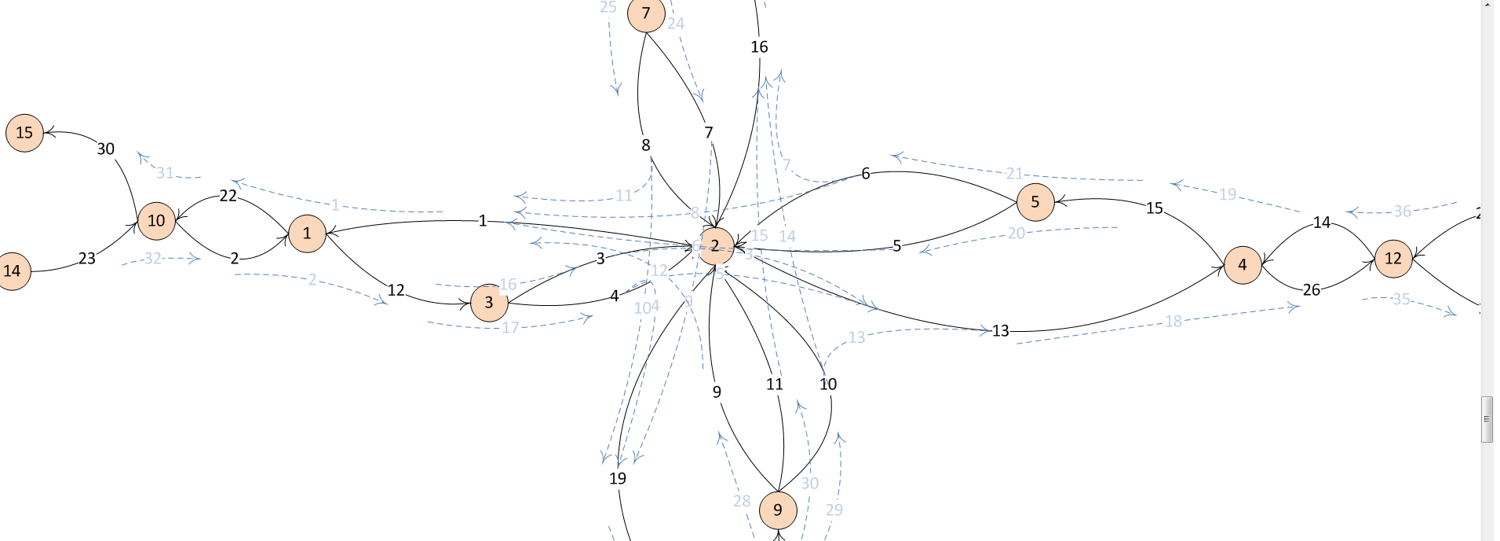
\includegraphics[scale=0.5]{GrafuDualny} 
\end{center}
\male
kluczowe są relacje skrętne a nie odcinki.
\end{frame}

\subsection{Opis stanu}
\begin{frame}{Opis stanu}{reprezentacja pojazdów w sieci drogowej}
\end{frame}


\begin{frame}{Pojazd (kierowca) mikroskopowy}{opis podstawowy}
\begin{center}
\includegraphics[scale=0.3]{mikro}
\end{center}
Pojazd $\alpha$ (kierowany przez kierowcę) w danej chwili czasu $t$ opisany jest (zazwyczaj) poprzez :
\begin{description}

\item[$x_{\alpha}(t)$] położenie pojazdu $\alpha$ w czasie $t$
\item[$v_{\alpha}(t)$] prędkość 
\item[$dv_{\alpha}(t)/dt$] zmianę prędkości 
\end{description}
\end{frame}

\begin{frame}{Pojazd (kierowca) mikroskopowy}{opis pełny}
Do opisu zachowania kierowcy (pojazdu) potrzebny jest opis stanu jego: $\alpha$ i innych: $\beta \in A$.
\\~\\
na podstawie których w miarę potrzeb oblicza się:
\\ $\dots$


\end{frame}

\begin{frame}{Pojazd (kierowca) mikroskopowy}{opis pełny}
\begin{center}
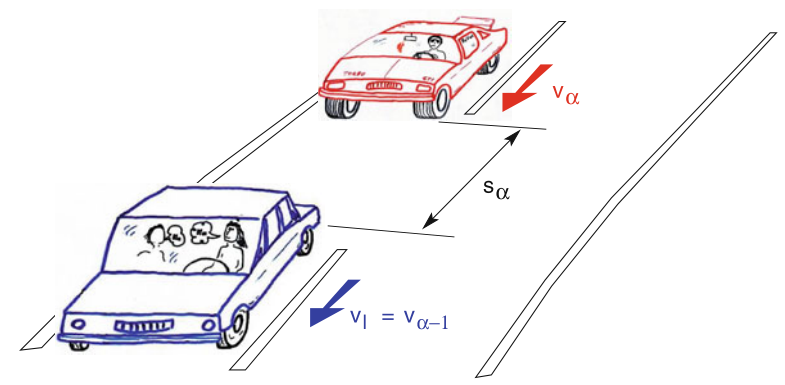
\includegraphics[scale=0.2]{CFM}
\end{center}
\male
Do modelowania zmiany położenia podłużenego (\textit{car-following model}) potrzebujemy dodatkowo opisu stanu pojazdu przed nami $x_{\alpha-1}$, jego: 
\begin{itemize}
\item położenia,
\item prędkości
\end{itemize}
czasami dodatkowo np. 
\begin{itemize}
\item jego przyśpieszenia d$v$/d$t$ 
\item informacji o włączeniu kierunkowskazu,
\item świateł stop.
\end{itemize}
~\\
Na podstawie tego obliczany jest odstęp $s$ [m] (\textit{bumber-to-bumper distance}):
\begin{equation*}
s_\alpha= x_{\alpha-1} - l_{\alpha-1} - x_{\alpha}
\end{equation*}
\end{frame}

\begin{frame}{Pojazd (kierowca) mikroskopowy}{opis pełny}
\begin{center}
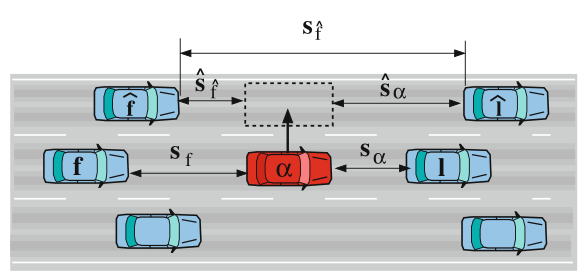
\includegraphics[scale=0.4]{laneChange}
\end{center}

Do modelowania \textbf{zmiany pasa}  (\textit{lane change }) potrzebujemy dodatkowo opisu stanu pojazdów przed i za nami na naszym pasie i na pasie docelowym (odstępy).
\end{frame}

\begin{frame}{Pojazd (kierowca) mikroskopowy}{opis pełny}
\begin{center}
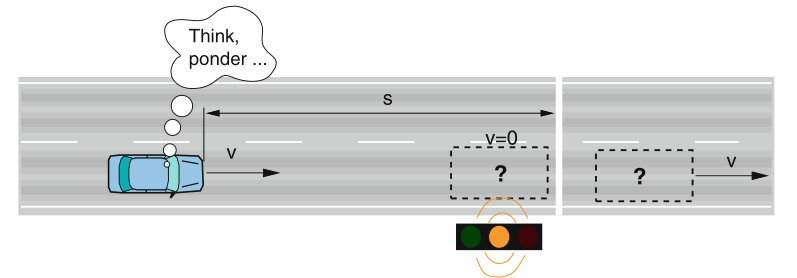
\includegraphics[scale=0.4]{Stoj}
\end{center}
Do decyzji o \textbf{zatrzymaniu} na sygnalizacji potrzebujemy odległości do linii zatrzymania $s$ w momencie zmiany fazy.
\end{frame}

\begin{frame}{Pojazd (kierowca) mikroskopowy}{opis stanu}
\begin{center}
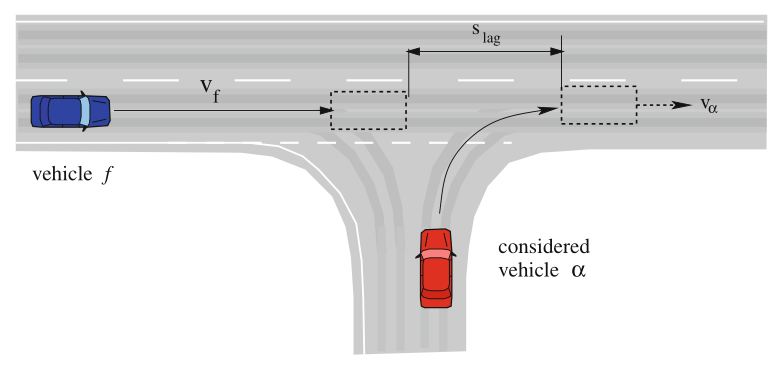
\includegraphics[scale=0.4]{Wlacz}
\end{center}
Do decyzji o \textbf{włączeniu} się na do ruchu skrzyżowaniu niesygnalizowanym potrzebujemy dodatkowo prędkości i odległości zbliżającego się pojazdu.
%\NumTabs(3)
%włącz \tab $\longleftarrow s_f > s_{bezp} (v_f,v_\alpha) \land s_{}$
\end{frame}

\begin{frame}{Pojazd (kierowca) mikroskopowy}{opis stanu}
\begin{center}
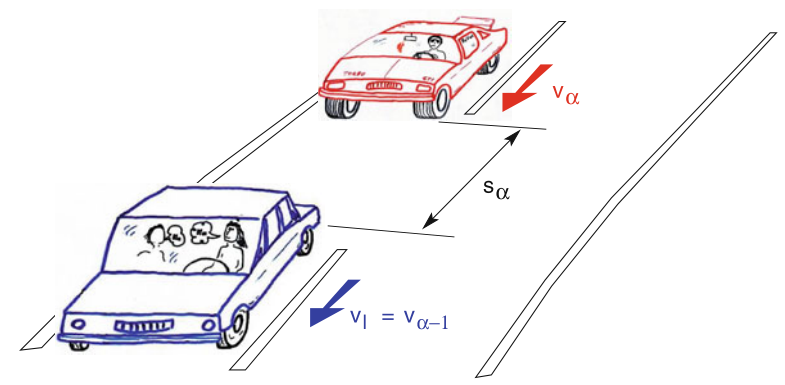
\includegraphics[scale=0.2]{CFM}
\end{center}
Kierowca (i pojazd) $\alpha$ w danej chwili czasu $t$ znajduje się w sytuacji (stanie) opisanej przez zmienne stanu, np.:
\begin{equation*}
(s_\alpha(t), v_\alpha(t), \dots)
\end{equation*} 
\male
dobór zmiennych zależy od rodzaju modelu i decyzji jaka jest podejmowana
\end{frame}

\subsection{Implementacje}
\begin{frame}{Implementacja}{algorytmy numeryczne symulujące ruch pojazdów}\end{frame}


\begin{frame}{Rodzaje implementacji}{modele ciągłe i dyskretne}

modele analityczne mogą być ciągłe - opisane są równaniami różniczkowymi i mogą byc obliczone dla dowolnej chwili czasu $t$, \\ w szczególności dla całego okresu symulacji $t \in T$. \\ Po prostu rozwiązuje się równanie różniczkowe \footnote{\bmale gdzie $a_{mic}$ to rezultat uzyskany z modelu mikroskopowego, który określimy później.} :
\begin{equation*}
\dot{v}_\alpha (t) = a_{mic}(s_\alpha, t_\alpha, v_l) 
\end{equation*}
ale komputery są binarne a nie ciągłe, wobec czego wszystkie implementacje na pewnym etapie muszą być zdyskretyzowane $t \in [0, 1 \cdot \Delta t , 2 \cdot \Delta t, \dots, t \cdot \Delta t]$:
\begin{equation*}
\dot{v}_\alpha (t+\Delta t) = a_{mic}(s_\alpha(t), v_\alpha(t), v_l(t))
\end{equation*}
określamy stan układu w kroku $t+\Delta t$ na podstawie stanu w kroku $t$. 
\end{frame}

\begin{frame}{Rodzaje implementacji}{modele ciągłe i dyskretne}
W implementacjach komputerowych (algorytmy) określamy stan układu w kroku $t+\Delta t$ na podstawie stanu w kroku $t$. 
Dwie możliwości:
\begin{enumerate}
\item $v_\alpha (t+\Delta t) = f(t)$ \\ proste rozwiązanie (symulacja krok po kroku)
\item $v_\alpha (t+\Delta t) = f(t+\Delta t)$ \\ kłopot (iteracyjne rozwiązanie w każdym kroku) (zagadnienie punktu stałego $x=f(x)$).
\end{enumerate}
Zazwyczaj mamy układ równań dolnoprzekątniowych, który można rozwiązać sekwencyjnie.
\end{frame}

\begin{frame}{Algorytm}{ogólny, dyskretny model mikrosymulacyjny}
\male
\begin{algorithm}[H]
\SetAlgoLined
 \KwIn{graf, dopływ pojazdów $\alpha$ z przypisaniem do ścieżek $k$}
  \Begin{
 $t\longleftarrow0$\\
  \If{$t \leq T$}{
   generuj dopływ pojazdów (na podstawie popytu i rozkładów p-wa na poszczególnych wlotach)\\
   $\alpha \longleftarrow 0$\\
   \While{$\alpha<A$}{
   określ położenie pojazdu $x_\alpha (t)$ - \textit{CFM, lane-change, gap acceptance} \\ 
   \If{koniec odcinka}
   {przejdź na kolejny odcinek na ścieżce $k$}   
   $\alpha \longleftarrow \alpha + 1$ \textit{kolejny pojazd} }
   $t \longleftarrow t + 1$\textit{kolejny krok czasu}
  }
\KwOut{trajektorie pojazdów  $X \longleftarrow \lbrace x_\alpha (t) : \alpha \in A \rbrace$} 
\textbf{opcjonalnie}: \textit{opracuj dodatkowe wyniki\footnote{\bmale np. straty czasu, długości kolejek, liczby zatrzymań}}}
\end{algorithm}
\end{frame}

\begin{frame}{Narzędzia}{przegląd}
\begin{enumerate}
\item komerycjne:
\begin{enumerate}
\item Synchro
\item Aimsun
\item Paramics
\item VISSIM
\item $\dots$
\end{enumerate}
\item badawcze
\begin{enumerate}
\item MATSim
\item dynaMIT
\item SUMO
\item Mezzo
\item Intelligent Driver Model \footnote{\bmale http://www.traffic-simulation.de}
\item Pawel Gora - \textit{Traffic Simulation Framework} \footnote{\bmale https://www.mimuw.edu.pl/$\sim$pawelg/indexpl.html}
\item $\dots$
\end{enumerate}
\end{enumerate}
\end{frame}




\subsection{Decyzje kierowcy}

\begin{frame}{Decyzje kierowcy}{przyśpiesz, zwolnij, zmień pas, czekaj, stój}
\end{frame}

\begin{frame}{Decyzje kierowcy}
kierowca podejmuje \textbf{decyzje} na podstawie opisu stanu:
\begin{itemize}
\item swojego ($v_\alpha,x_\alpha,a_\alpha$)
\item innych pojazdów (odległości, różnice prędkości)
\item przeszkód (np. czerwone światło)
\end{itemize}
\end{frame}


\begin{frame}{Decyzje kierowcy}{rodzaje decyzji}
\begin{center}
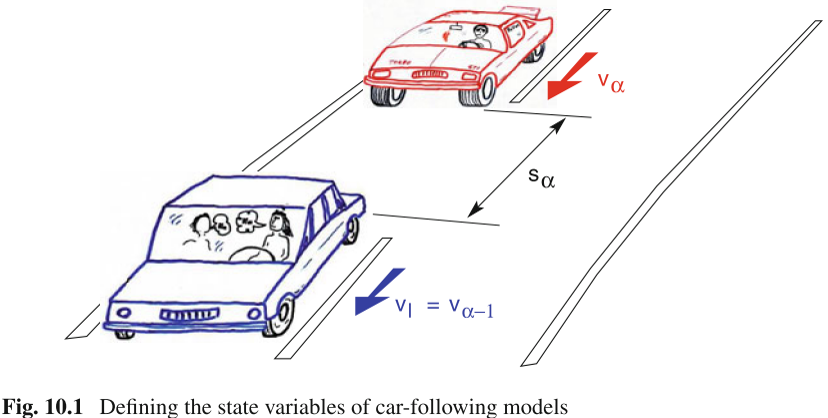
\includegraphics[scale=0.3]{CF1}
\end{center}
\male
\begin{itemize}
\NumTabs{3}
\item podążanie za liderem \tab \textbf{ciągła} decyzja o przyśpieszeniu lub hamowaniu
\item zmiana pasa \tab \textbf{dyskretna} decyzja o położeniu poprzecznym
\item włączenie się do ruchu \tab \textbf{dyskretna} decyzja ruszam/czekam, zatrzymuję się/jadę
\end{itemize}
\end{frame}


\subsection{Podążanie za liderem}
\begin{frame}{Podążanie za liderem}{opis}
\begin{center}
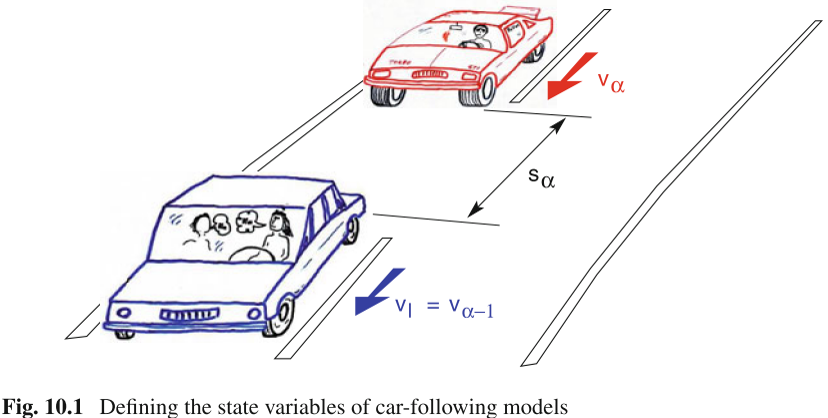
\includegraphics[scale=0.2]{CF1}
\end{center}
\male
Zmienne decyzyjna to \textbf{przyśpieszenie} $\dot{v}_\alpha (t)$, $a_\alpha (t)$.\\~\\
W ujęciu dyskretnym określam prędkość w kolejnym kroku $t+\Delta t$ na podstawie aktualnego opisu stanu:
\begin{equation*}
v_\alpha (t+\Delta t) = v_{mic}(s_\alpha(t), v_\alpha(t), v_l(t))
\end{equation*}
\\~\\~\\
Położenie $x_\alpha$ jest zazwyczaj interpolowane:
\begin{equation*}
x_\alpha (t+\Delta t)=x_\alpha (t)+\frac{v_\alpha (t)+v_\alpha (t+ \Delta t)}{2}\Delta t
\end{equation*}
\end{frame}

\begin{frame}{Podążanie za liderem}{stan równowagi \textit{cruise}}
\begin{center}
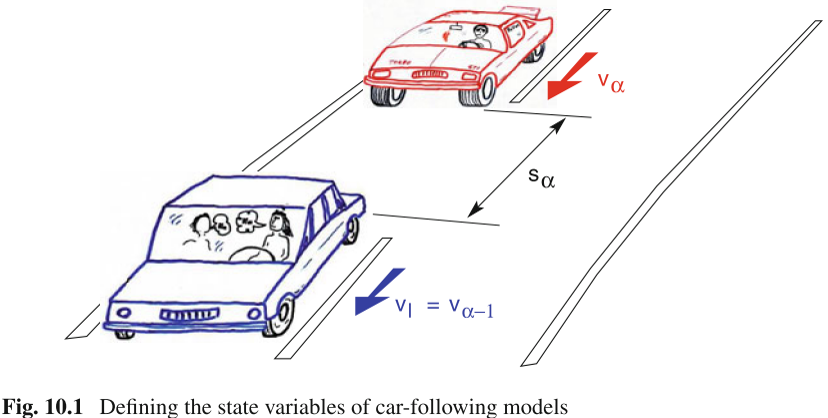
\includegraphics[scale=0.2]{CF1}
\end{center}
\NumTabs{3}
wszystkie pojazdy jadą z tą samą prędkością \tab $v_\alpha = v_\beta$ : $\forall \alpha, \beta \in A$
\\w takich samych odstępach \tab $s_\alpha = s_\beta$ : $\forall \alpha, \beta \in A$
\\ i nie przyśpieszają \tab \tab  $a_\alpha = 0$ : $\forall \alpha \in A$
\end{frame}

\begin{frame}{Podążanie za liderem}{stan nierównowagi}
\begin{center}
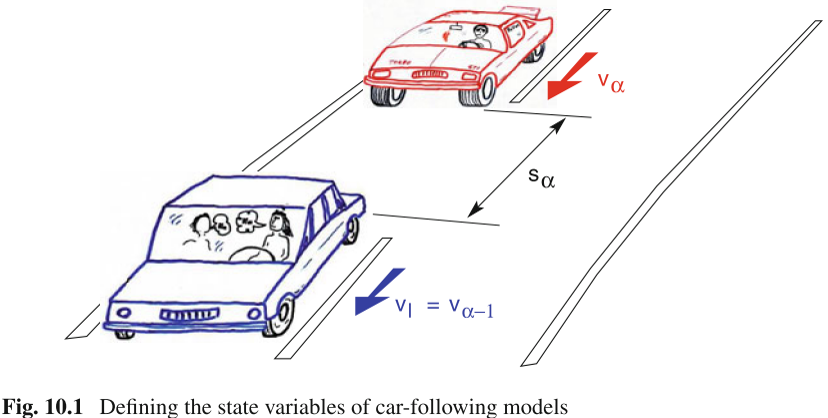
\includegraphics[scale=0.2]{CF1}
\end{center}
konieczność decyzji o zmianie prędkości, np.\\ \alert{Intelligent Driver Model (IDM)}
\begin{equation*}
\dot{v}=a \left[ 1- \left( \frac{v}{v_0} \right) ^\delta - \left( \frac{s^*(v,\Delta v)}{s} \right) ^2 \right]
\end{equation*}
\begin{equation*}
s^*(v,\Delta v) = s_0 + max \left( 0, vT + \frac{v \Delta v}{2 \sqrt{ab}} \right)
\end{equation*}
\end{frame}

\begin{frame}{Podążanie za liderem}{IDM}
\begin{equation*}
\dot{v}=a \left[ 1- \left( \frac{v}{v_0} \right) ^\delta - \left( \frac{s^*(v,\Delta v)}{s} \right) ^2 \right]
\end{equation*}
\begin{equation*}
s^*(v,\Delta v) = s_0 + max \left( 0, vT + \frac{v \Delta v}{2 \sqrt{ab}} \right)
\end{equation*}
\bmale 
gdzie: \\~\\\begin{center}

\begin{tabular}{cccc}
\hline 
parametr & opis & typowa wartość (zamiejska) &  (miejska) \\ 
\hline 
$v_0$ & pożądana prędkość & 120km/h & 54 km/h \\ 
$\delta$ & parametr profilu przyśpieszenia & 4 & 4 \\ 
$s_0$ & minimalny odstęp & 2m & 2m \\ 
$a$ & przyśpieszenie & 1$m/s^2$ & 1$m/s^2$ \\ 
$b$ & opóźnienie & 1.5$m/s^2$ & 1.5$m/s^2$ \\ 
$T$ & czas reakcji & 1s & 1s \\ 
\hline 
\end{tabular}
\end{center}
\end{frame}

\begin{frame}{Podążanie za liderem}{IDM - wyniki}
\male IDM\\
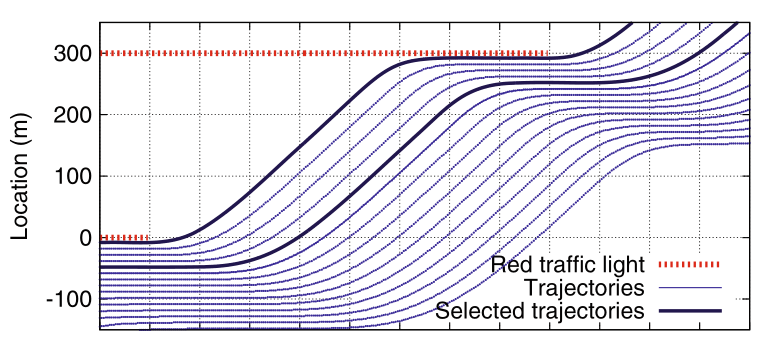
\includegraphics[scale=0.4]{IDM}\\
\male vs. model pierwszego rzędu\\
~~~~~~~~~~~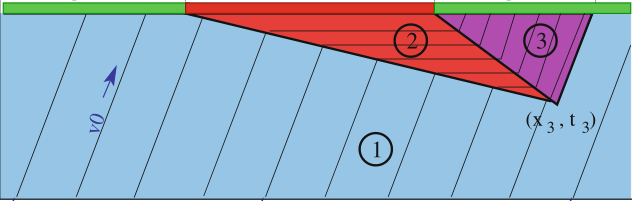
\includegraphics[scale=0.4]{pierwszy}
\end{frame}

\begin{frame}{Podążanie za liderem}{Model Wiedemann'a}
Model opisuje psychofizyczne zachowanie kierowcy w czterech reżimach:
\begin{enumerate}
\item ruch niezakłócony
\item zbliżanie się do wolniejszego pojazdu
\item podążanie za liderem (nie ma pełnej równowagi, są ciągłe oscylacje)
\item krytyczne sytuacje wymagające hamowania.
\end{enumerate}
w każdym z nich używane są inne funkcje: $a_\alpha  = a_{mic}(s, v, \Delta v)$.
\end{frame}

\begin{frame}{Podążanie za liderem}{Model Wiedemann'a - wykres reżimów}
\begin{center}
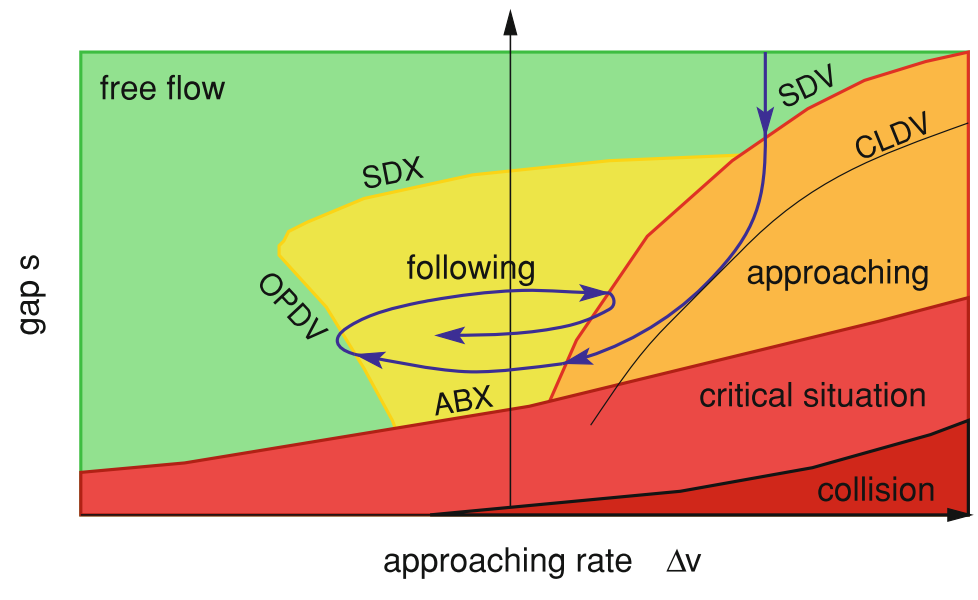
\includegraphics[height=5cm]{WiedemannGraf}
\end{center}
\male
\NumTabs{4}
\alert{SDV} \tab próg czułości (zaczynam zwalniać)\\
\alert{CLDV} \tab optymalny odstęp (do takiej odległości chcę zwolnić)\\
\alert{OPDV} \tab próg rozjeżdżania (zaczynam przyśpieszać)\\
\alert{ABX} \tab minimalny (ściśle) odstęp przy podążaniu za liderem\\
\alert{SDX} \tab maksymalny (nie ściśle) odstęp przy podążaniu za liderem\\
\end{frame}

\begin{frame}{Podążanie za liderem}{Dostępne modele}
\male
\begin{itemize}
\item Optimal Velocity Model
\item Newell's Car Following Model
\item Gipp's Model
\item Intelligent Driver Model
\item Wiedemann Model
\item Nagel-Schreckenberg Model
\item Barlovic Model
\item $\dots$
\end{itemize}
\end{frame}


\subsection{Sytuacje dyskretne}
\begin{frame}{Sytuacje dyskretne}{wybór opcji}
\end{frame}

\begin{frame}{Sytuacje dyskretne}{ogólnie}
\male
Kierowca wybiera opcję $k$ spośród dostępnych opcji $K$. \\~\\
Opcje:
\begin{enumerate}
\item zmiana pasa: zostań/zmień
\item zatrzymanie na światłach: zatrzymuj się/przejedź
\item wlot podporządkowany: czekaj/jedź.
\end{enumerate}~\\~\\
Wybór jest ograniczony przez \alert{kryterium bezpieczeństwa}, tj. żaden inny kierowca $\beta$ nie powinien w wyniku naszej decyzji $k$ być zmuszonym do hamowania z przyśpieszeniem większym niż $b_{\mathrm{safe}}$ (ok. 2$m/s ^2$):
\begin{equation*}
\alpha_(\beta, k) < b_{\mathrm{safe}}
\end{equation*}

Wybiera w oparciu o kryterium największej (\alert{subiektywnej}) użyteczności $U^{\alpha, k}$:
\begin{equation*}
k^*= \argmax_{k \in K} U^{\alpha, k}
\end{equation*}
\end{frame}

\begin{frame}{Zmiana pasa}{kryterium z IDM}
\begin{center}
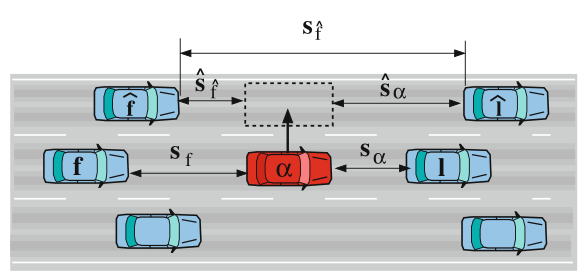
\includegraphics[height=3cm]{laneChange}\\
\end{center}
Sprawdź czy odstęp na sąsiednim pasie $s_{\hat{f}}$ jest wystarczający. Np. (IDM):
\male
\begin{equation*}
s_{\hat{f}} > s^{\mathrm{IDM}}_{\mathrm{safe}} = \frac{s^* (v_{\hat{f}}, v_{\hat{f}}-v_\alpha)}{\sqrt{\frac{b_{\mathrm{safe}}}{a} }}
\end{equation*}
\end{frame}

\begin{frame}{Zmiana pasa}{kryterium z IDM}
\begin{center}
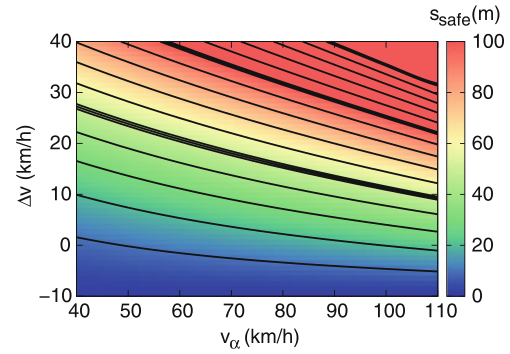
\includegraphics[height=5cm]{Safe}\\
\end{center}
wartości bezpiecznego odstępu w zależności od prędkości $v$ i różnicy prędkości $\Delta v$ obliczone w IDM.
\end{frame}

\begin{frame}{Zmiana pasa}{model ogólny}
\begin{figure}
\begin{center}
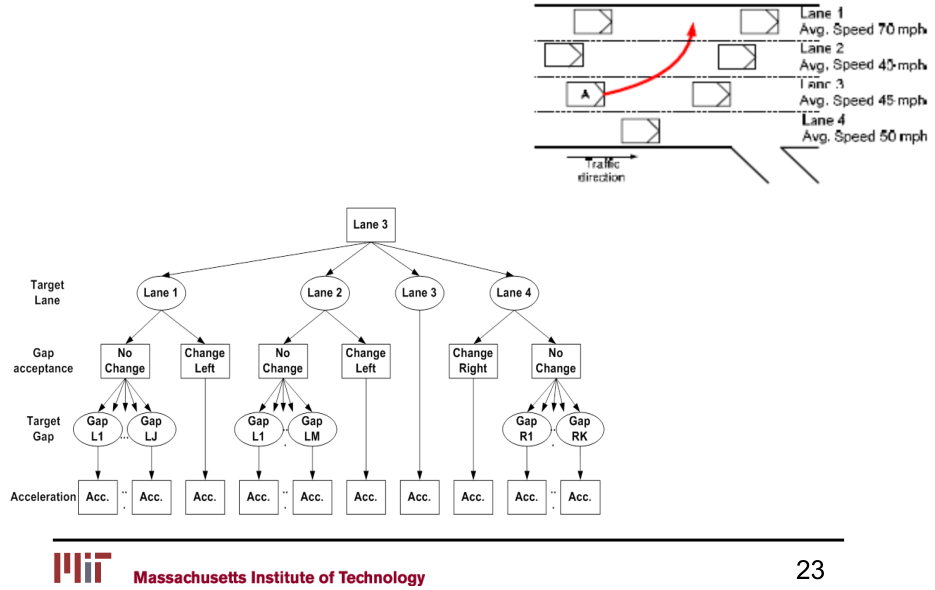
\includegraphics[scale=0.4]{MIT}
 \caption{\bmale źródło: M. Ben-Akiva, MIT Course 2014}
\end{center}
\end{figure}
\end{frame}

\begin{frame}{Zatrzymanie się na światłach}{kryterium z IDM}
\begin{center}
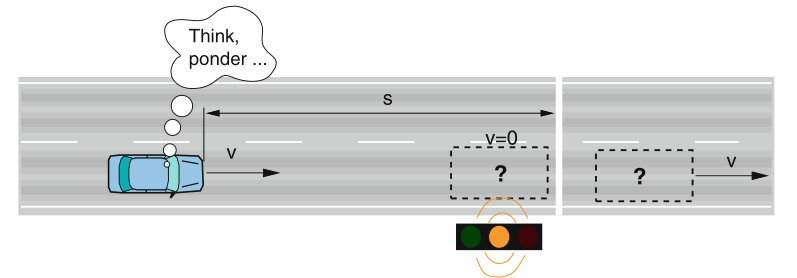
\includegraphics[height=4cm]{Stoj}\\
\end{center}
\NumTabs{4}
jedź\footnote{\male jeśli musiałbyś hamować z opóźnieniem większym niż  $b_{\mathrm{safe}}$} \tab jeśli $a_\alpha < - b_{\mathrm{safe}}$ 
\\ stój \tab w przeciwnym wypadku
\end{frame}

\begin{frame}{Włączanie się do ruchu}{kryterium z IDM}
\begin{center}
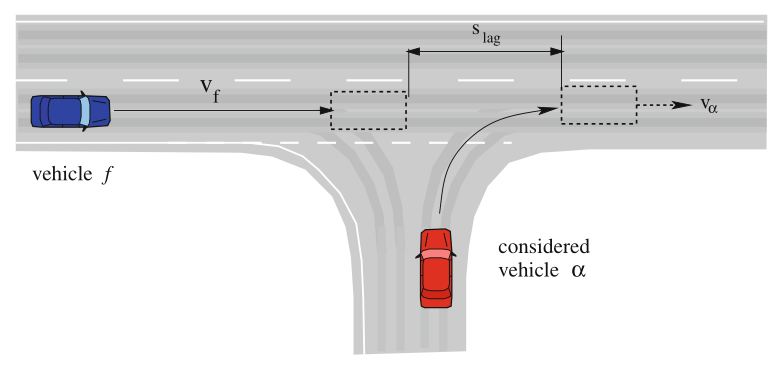
\includegraphics[height=3cm]{Wlacz}\\
\end{center}
Tutaj można stosować kryterium zmiany pasa odpowiednio podmieniając zmienne.
\NumTabs{4}\\
włącz się \tab jeśli $s_{\mathrm{lag}}> s_{\mathrm{sefe}}$ 
\\ poczekaj \tab w przeciwnym wypadku
\end{frame}

\subsection{Zachowanie kierowcy}
\begin{frame}{Zachowanie kierowcy}{szacowanie zmiennych stanu, reakcje, decyzje}
\end{frame}
\begin{frame}{Zachowanie kierowcy}{charakterystyka}
\male
Kierowca w rzeczywistości:
\begin{enumerate}
\item ma skończony (dodatni) czas reakcji,
\item popełnia błędy w ocenie sytuacji (np. przeszacowuje odległość),
\item ma zdolności strategiczne (potrafi przewidzieć sytuacje i zareagować na nią z wyprzedzeniem), 
\item odczytuje sygnały od innych kierowców (klaskon, kiwnięcie głowa, brzydkie słowo, niepewny tor jazdy, ...),
\item buduje swoją długofalowa strategie (po kilku latach stania w korku ma swoje techniki - subiektywnie optymalne),
\item niewrażliwość na małe zmiany $\Delta v \sim 0$ jest niezauważalna,
\item jest uprzejmy i dba o innych, lub wręcz przeciwnie (system kooperacyjny o \textit{quasi-}globalnym optimum, albo \textit{user-optimum}),
\end{enumerate}
\end{frame}

\begin{frame}{Zachowanie kierowcy}{reakcja}
\male
Kierowca \textbf{reaguje} na zmiany stanu ruchu drogowego, ale reakcja trwa ($T_r$). \\~\\

Proces reakcji kierowcy, $T_r= \sum$:
\begin{enumerate}
\item reakcja mentalna: \\ \quotedblbase widzę obiekt na drodzę \textquotedblright $\rightarrow$ \quotedblbase rozpoznaję, że to człowiek\textquotedblright $\rightarrow$ \quotedblbase identyfikuję zagrożenie \textquotedblright $\rightarrow$ \quotedblbase wybieram optymalną decyzję \textquotedblright $\rightarrow$ \quotedblbase hamuję/skręcam/nic nie robię \textquotedblright
\item czas czynności: \\ ruch nogą do hamulca, mocniejsze ściśnięcie kierownicy, odstawienie kawy
\item czas reakcji pojazdu: \\ zależny od systemu układu hamulcowego czas na faktyczne rozpoczęcie hamowania.
\end{enumerate}
~\\Wobec tego podstawowe równanie:
\begin{equation*}
\dot{v}_\alpha (t+\Delta t) = a_{mic}(s_\alpha(t), v_\alpha(t), v_l(t))
\end{equation*}
przyjmuje bardziej realistyczną postać:
\begin{equation*}
\dot{v}_\alpha (t+\Delta t) = a_{mic}\left( s_\alpha(t-T_r), v_\alpha(t-T_r), v_l(t-T_r) \right)
\end{equation*}
\end{frame}

\begin{frame}{Zachowanie kierowcy}{błędy w ocenie sytuacji}
Opis stanu (własnego i innych pojazdów) jest subiektywny. Zależy od kierowcy i może być błędny, dlatego w rzeczywistości kierowca podejmuje decyzje na podstawie subiektywnych wartości zmiennych stanu, a nie obiektywnych
\begin{equation*}
s_\alpha(t) \rightarrow s^{est}_\alpha(t)
\end{equation*}
\end{frame}

\begin{frame}{Zachowanie kierowcy}{błędy w ocenie sytuacji}
Błąd $| s_\alpha(t) - s^{est}_\alpha(t)|$ jest zmienną losową. 
\\
W najprostszym przypadku może być opisany rozkładem normalnym:
\begin{equation*}
| s_\alpha(t) - s^{est}_\alpha(t)|  \sim N(0,1)
\end{equation*}
W bardziej realistycznym opisie może to być np. proces Wienera\footnote{ \bmale czyli losowość ale o spójnym przebiegu w czasie. Przy użyciu wprost rozkładu normalnego (biały szum) kierowca może w chwili $t$ przeszacować, a w chwili $t+ \Delta t$ niedoszacować, proces Wienera jest bardziej spójny i kierowca albo konsekwentnie niedoszacowuje albo konsekwentnie przeszacowuje.}
\begin{center}
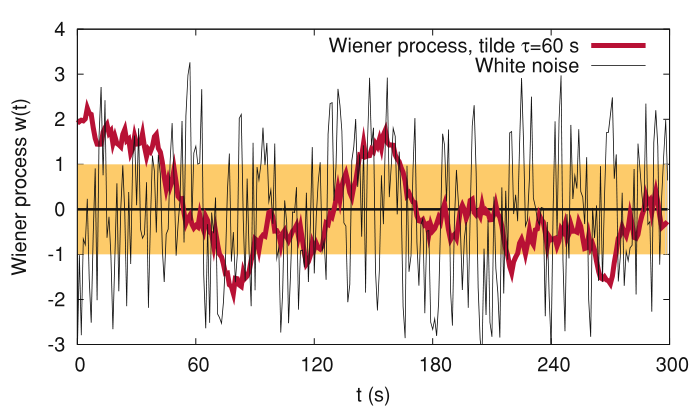
\includegraphics[scale=0.35]{Wiener}
\end{center}
\end{frame}

\begin{frame}{Zachowanie kierowcy}{powstawanie stop \& go wave}
\begin{columns}
\column{0.4\textwidth}
zaburzenie płynności pierwszego pojazdu eskaluje i powoduje coraz większe oscylacje
\column{0.6\textwidth} 
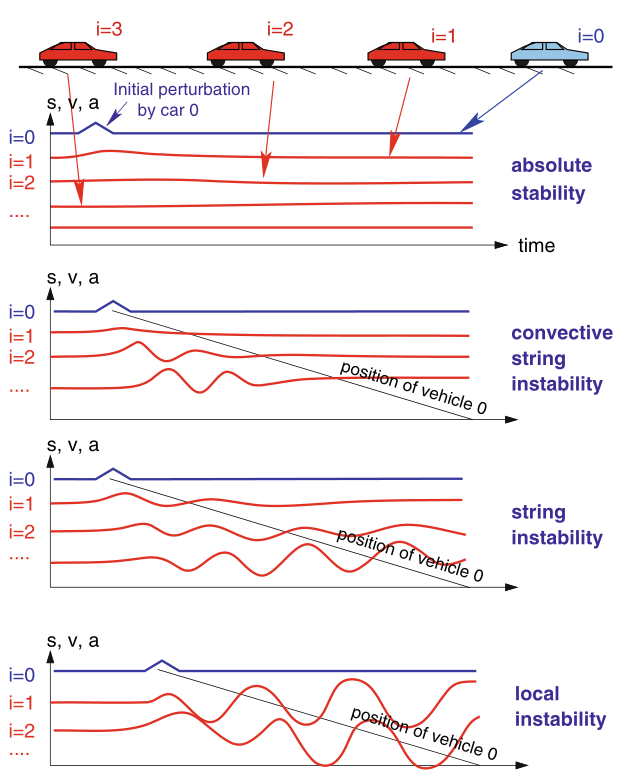
\includegraphics[scale=0.3]{SandG}
\end{columns}
\end{frame}

\begin{frame}{Zachowanie kierowcy}{przewidywanie}
Kierowca przewiduje na kilka kroków wprzód.
Jak to uwzględnić w modelu mikroskopowym? (otwarte pytanie \alert{MITSIM})
\begin{figure}
\begin{center}
 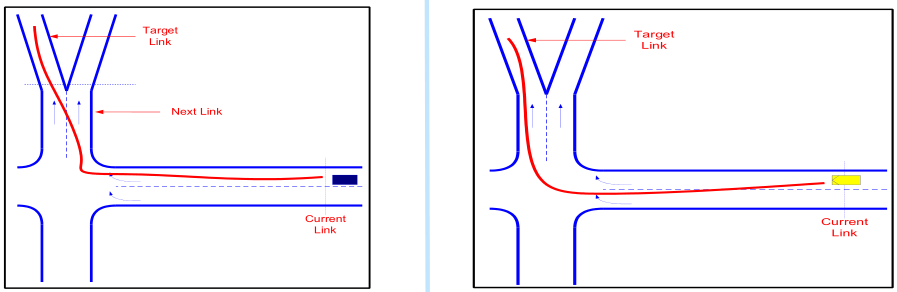
\includegraphics[height=3cm]{Przew}
 \caption{\bmale źródło: M. Ben-Akiva, MIT Course 2014}
\end{center}
\male kierowca nieprzewidujący (z lewej) i przewidujący (z prawej)
\end{figure}
\end{frame}




\subsection{Wyniki}
\begin{frame}{Wyniki symulacji}{jak je przedstawić, interpretować i używać}
\end{frame}

\begin{frame}{Wyniki symulacji}{pierwotne}
ogólnie: $ \lbrace x_\alpha (t) : \alpha \in A , t \in T \rbrace$
\begin{center}
 \includegraphics[scale=0.3]{trajektorie1}\\
\end{center}
\male zbiór pełnych trajektorii wszystkich pojazdów
\end{frame}

\begin{frame}{Wyniki symulacji}{przetworzone}
\begin{columns}
\column{0.5\textwidth}
\male
na podstawie trajektorii można określić następujące miary mikroskopowe:
  \begin{itemize}
  \item czas przejazdu pomiędzy zadanymi punktami.
  \item liczba zatrzymań
  \item prędkość
  \item strata czasu (czas z zatrzymaniami minus czas bez zatrzymań).
  \item emisja
  \item $\dots$
  \end{itemize}
  \column{0.5\textwidth}
 \includegraphics[scale=0.3]{trajektorie1}
 \end{columns}
\end{frame}

\begin{frame}{Wyniki symulacji}{wyniki makro (zagregowane)}
\begin{columns}
\column{0.5\textwidth}
\male
Wyniki mikro możemy agregować do \\ \textbf{rozkładu zmiennej losowej (średnia, kwantyle, maksymalne i minimalne)}, \\ np:
  \begin{itemize}
  \item czas przejazdu 
  \item długość kolejki
  \item straty czasu
  \end{itemize}
  itp.
    \column{0.5\textwidth}
 \includegraphics[scale=0.3]{pdf}
 \end{columns}
\end{frame}

\begin{frame}{Wyniki symulacji}{interpretacja}
\begin{columns}
\column{0.7\textwidth}

np. długość kolejki:
\begin{itemize}
\item średnia z symulacji:
\begin{itemize} 
\item średnia z całej symulacji \\ $\bar{l}_t:t \in T$ 
\item średnia z symulacji bez początków i końców (\textit{warm-up, cool-down}): \\ $\bar{l}_t:t \in T'$
\item maksimum, mediana, kwantyl (jaki?)
\item odchylenie standardowe
\end{itemize}
\item średnia z kilku symulacji
\begin{itemize} 
\item średnia ze średnich z kilku symulacji
\item średnia z kwantyli z kilku symulacji
\end{itemize}
\end{itemize}
    \column{0.3\textwidth}
 \includegraphics[scale=0.2]{pdf}
 \end{columns}
\end{frame}

\begin{frame}{Wyniki symulacji}{liczba symulacji}
\male
Podstawowe narzędzia statystyki: dobór liczebności próby $n$ dla oszacowania rozkładu zmiennej losowej.
\\
\begin{itemize}
\item określamy charakterystykę, którą chcemy oszacować (np. czas przejazdu, długość kolejki)
\item czy interesuje nas średnia, odchylenie, czy kwantyl?
\item określamy przedział i poziom ufności $u$ np. $d$ na poziomie ufności $\alpha$ = 90\% - z odwrotnej dystrybuanty rozkładu normalnego.
\item wykonujemy kilka ($n$) symulacji i obliczamy odchylenie standardowe $\sigma$ interesującej nas charakterystyki 
\end{itemize}
liczba replikacji:
\begin{equation*}
n \geq u^2_{1-\alpha / 2} \cdot \frac{ \sigma^2}{d^2}
\end{equation*}
zazwyczaj kilkadziesiąt
\end{frame}

\begin{frame}{Wyniki symulacji}{graficznie}
\begin{figure}
\begin{center}
 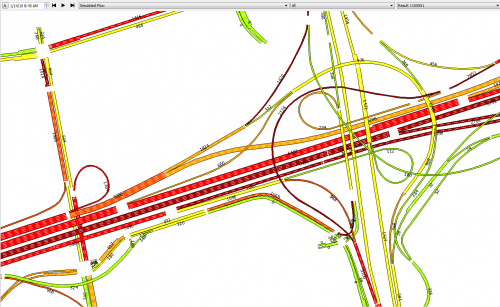
\includegraphics[height=3cm]{Aimsun}
 \caption{\bmale źródło: AIMSUN}
\end{center}
\end{figure}
\male
kolorowanie grafu zgodnie z wartością charakterystyki:
\begin{itemize}
\item prędkość (średnia, dolny kwantyl, odchylenie, $\dots$)
\item potok (poj./s)
\item długość kolejki
\item czas przejazdu
\item gęstość
\item emisja
\item $\dots$
\end{itemize}
i ich ewolucja w czasie: $\cdot(t)$
\end{frame}


\begin{frame}{Wyniki symulacji}{zakres czasowy}
Sieć musi się rozgrzać (\alert{warm-up}) i dopiero z rozgrzanej sieci możemy zbierać wyniki.
\begin{figure}
\begin{center}
 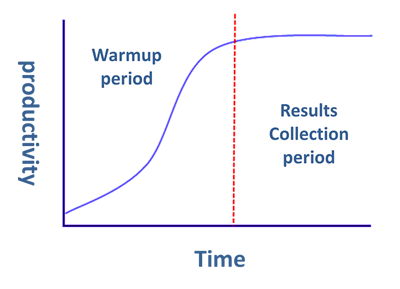
\includegraphics[height=3cm]{WarmUp}
 \caption{\bmale źródło: Simul8.com}
\end{center}
\end{figure}
\male
Np. Gdy chcemy symulować godzinę szczytu porannego (8-9) to symulacja nie może się zacząć od pustej sieci, bo sieć przed ósmą nie jest pusta (są kolejki, mniejsze ale są)
\end{frame}

\begin{frame}{Wyniki symulacji}{zakres czasowy}
Zazwyczaj chcemy uzyskać wyniki symulacji dla godziny (np. szczytu porannego $8-9$), ale co to znaczy w modelu dynamicznym?
\\~\\~\\
\begin{columns}
\column{0.5\textwidth}
\male
Możliwe interpretacje godziny szczytu:
\begin{itemize}
\item pojazdy generowane pomiędzy $8-9$ i tylko te pojazdy są symulowane, mogą dojechać później.
\item pojazdy generowane pomiędzy $8-9$ przy czym wszystkie pojazdy są symulowane również te wyjeżdżające wcześniej i później.
\item części trajektorii wszystkich pojazdów pomiędzy $8-9$ (tylko części trajektorii są brane pod uwagę)
\item pojazdy przejeżdżające przez analizowany obszar pomiędzy $8-9$ w tym te które rozpoczęły podróż wcześniej (tylko części trajektorii są brane pod uwagę i tylko w obszarze).
\end{itemize}
\column{0.5\textwidth}
 \includegraphics[scale=0.4]{trajektorie1}
\end{columns}
\end{frame}


\subsection{Kalibracja}
\begin{frame}{Kalibracja}{zgodność modelu z rzeczywistością}
\end{frame}

\begin{frame}{Kalibracja}{}
\alert{kalibracja} to proces ustalenia postaci i parametrów modelu. Jego celem jest maksymalizacja zgodności modelu z rzeczywistością.

~\\
\alert{rzeczywistość} musimy miec zaobserwowaną: zmierzoną i opisaną (np. zapis wideo, pętle indukcyjne, pojazdy sondujące, długości kolejek).
~\\
\alert{zgodność} musimy mierzyć i maksymalizować $\rightarrow$ problem optymalizacyjny.

\end{frame}

\begin{frame}{Kalibracja}{znaczenie}
np. przeszacowanie czasu reakcji\\
\begin{figure}
\begin{center}
 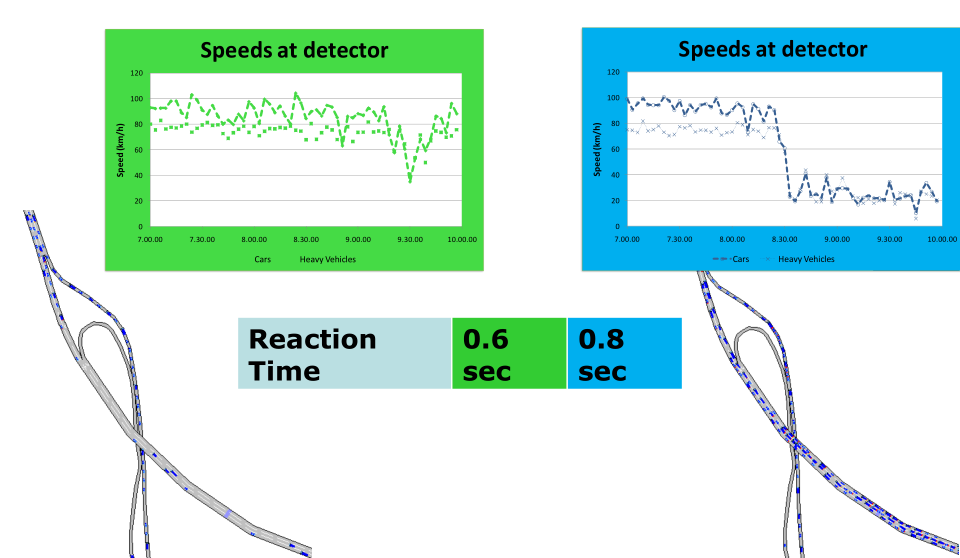
\includegraphics[height=5cm]{Punzo}
 \caption{\bmale źródło: V. Punzo, MIT Course 2014}
\end{center}
\end{figure}
\end{frame}

\begin{frame}{Kalibracja}{problem optymalizacyjny}
\male
Dopasowanie:\\
\begin{equation*}
S( \bm{\beta} ) = \sum^n_{i=1} || y^{sim}_i(\bm{\beta}) - y^{data}_i(\bm{\beta}) ||
\end{equation*}
gdzie:

\begin{description}
\item[$S$] to miara dopasowania
\item[$\bm{\beta}$] to wektor parametrów modelu
\item[$n$] to liczba obserwacji
\item[$y^{sim}_i$] to wynik modelu
\item[$y^{data}_i$] to wynik pomiaru
\item[$||~||$] to ogólna miara dopasowania (np. SSE, MSE, RMSE, $(x-\hat{x})^2$, $\dots$)
\end{description}
~\\
Problem optymalizacyjny:
\begin{equation*}
\hat{\bm{\beta}}= \argmin_{\bm{\beta}} S(\bm{\beta})
\end{equation*}
\end{frame}

\begin{frame}{Kalibracja}{dopasowanie modelu w skali mikro}
zgodność rzeczywistego zjawiska (w skali mikro) z modelowanym (w skali mikro)
\\~\\
profil przyśpieszenia pojedynczego pojazdu $\dot{v}_\alpha (t)$:\\
\begin{center}
\includegraphics[scale=0.3]{acc}
\end{center}
\end{frame}

\begin{frame}{Kalibracja}{dopasowanie modelu w skali mikro}
wyniki kalibracji modelu \alert{parametryzacja}:\\ \male wartości parametrów i rozkładów.
\begin{figure}
\begin{center}
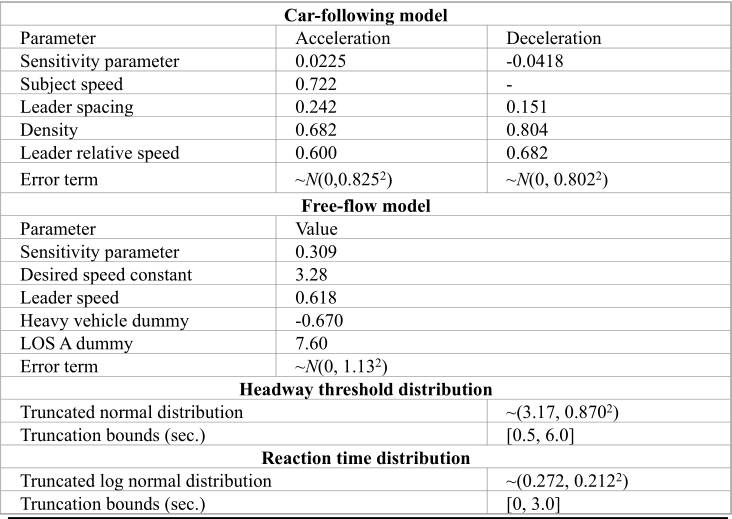
\includegraphics[height=5cm]{Estym}
 \caption{\bmale źródło: Ahmed, 1999}
\end{center}
\end{figure}
\end{frame}

\begin{frame}{Kalibracja}{dopasowanie modelu w skali makro}
zgodność rzeczywistego stanu sieci (w skali makro) z modelowanym (w skali makro)
\\~\\
wykres droga-prędkość-czas:
\begin{center}
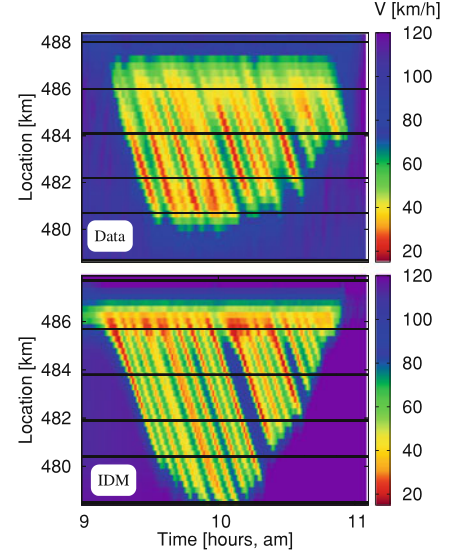
\includegraphics[scale=0.3]{KalibMakro}
\end{center}
\end{frame}

\begin{frame}{Kalibracja}{weryfikacja ogólna}
zgodność wartości globalnych:
\\~\\
np. liczba pojazdów $N$
\begin{figure}
\begin{center}
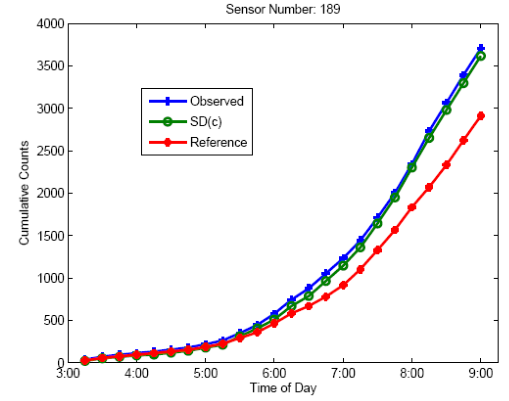
\includegraphics[scale=0.3]{MBA}
 \caption{\bmale źródło: M. Ben-Akiva, MIT Course 2014}
\end{center}
\end{figure}
\end{frame}


\subsection{Sygnalizacja i sterowanie w modelowaniu mikroskopowym}

\begin{frame}{Sygnalizacja i sterowanie w modelowaniu mikroskopowym}{kontrola przepływu pojazdów}
\end{frame}

\begin{frame}{Sygnalizacja w modelowaniu mikroskopowym}{sposób odwzorowania}
w trzonie modelu sytuacja jest \alert{zerojedynkowa}:

\begin{description}
 \item[czerwone] stój
 \item[zielone] jedź
 \end{description}

$\dot{v}_\alpha (t) = a_{mic}(s_\alpha, t_\alpha, v_l, \bm{signal})$
\\
w praktyce to kilka linii kodu w algorytmie bazowym

\end{frame}

\begin{frame}{Sygnalizacja}{upraszczanie}
Po stronie samego modelu nie ma znaczenia jaki i jak bardzo skomplikowany jest plan sygnalizacji.
\begin{columns}
\column{0.5\textwidth}
 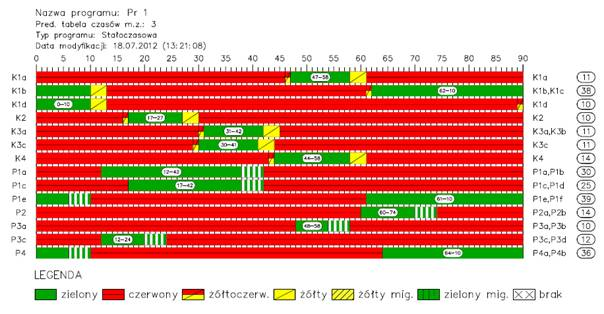
\includegraphics[scale=0.3]{fazy}
\column{0.5\textwidth}
\includegraphics[scale=0.3]{algorytm}
\end{columns}

i tak upraszczamy go do informacji przekazanej kierowcy: \alert{zielone|czerwone}
\end{frame}

\begin{frame}{Sterowanie}{realistyczny model}
dzięki realizmowi modelu mikroskopowego nie potrzebujemy metod do odwzorowania systemów sterowania, po prostu budujemy je identyczne jak w rzeczywistości.
\\~\\
co więcej modele mikroskopowe stosujemy jako środowiska do testowania systemów zarządzania, sygnalizacji akomodacyjnej, koordynacji, itp. \\~\\
\alert{ale to nie jest element symulacji mikroskopowej}.
\begin{center}
\begin{columns}
\column{0.4\textwidth}
 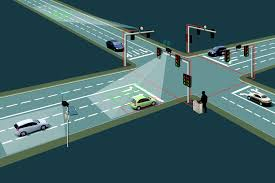
\includegraphics[scale=0.5]{detekcja}
\column{0.6\textwidth}
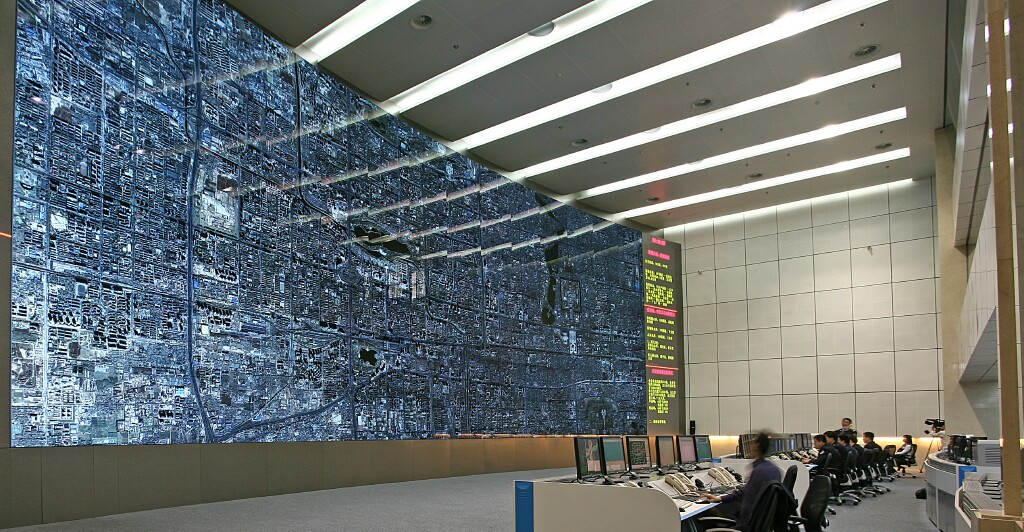
\includegraphics[scale=0.17]{ITS}
\end{columns}
\end{center}
\end{frame}


\begin{frame}{Sterowanie}{możliwości zastosowania modelu}
model symuluje przepływ pojazdów (kierowców w pojazdach) przez sieć. \\
możemy symulować np.:
\male
\begin{itemize}
\item wpływ znaków zmiennej treści na trasę
\item testować sterowanie obszarowe
\item testować priorytetowanie (uprzywilejowane, komunikacja zbiorowa)
\item testować pojazdy autonomiczne
\item badać wpływ aplikacji mobilnych (nawigacja w czasie rzeczywistym)
\item kooperacje pomiędzy pojazdami autonomicznymi
\item minimalizować emisję
\item itp.
\end{itemize}
\end{frame}


\subsection{Popyt w modelu mikroskopowym}

\begin{frame}{Popyt}{odzwierciedlenie przepływu pojazdów przez sieć}
\end{frame}

\begin{frame}{Popyt}{generacja pojazdów}
Dwie opcje:
\begin{itemize}
\item \alert{explicit:} ścieżki $k$ i popyt na nich $q_k$\\
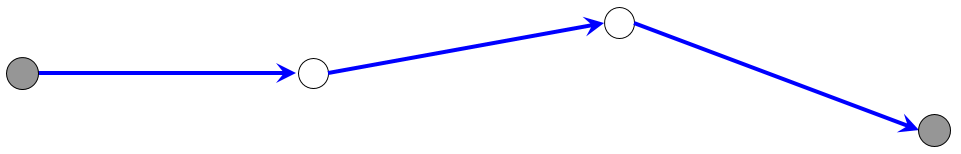
\includegraphics[height=1cm]{path}
\item \alert{implicit:} generacja na wlocie $q_a$ i rozploty w punktach decyzyjnych $r_a(t)$ \\
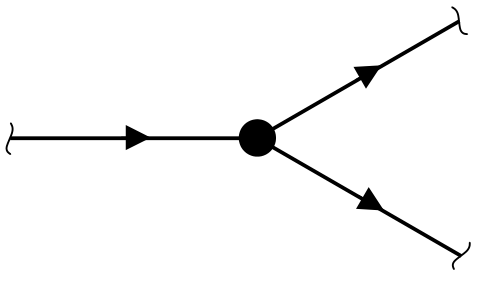
\includegraphics[height=2cm]{SR}
\end{itemize}
\end{frame}

\begin{frame}{Popyt}{pojazdy podążające po ścieżkach}
\begin{center}
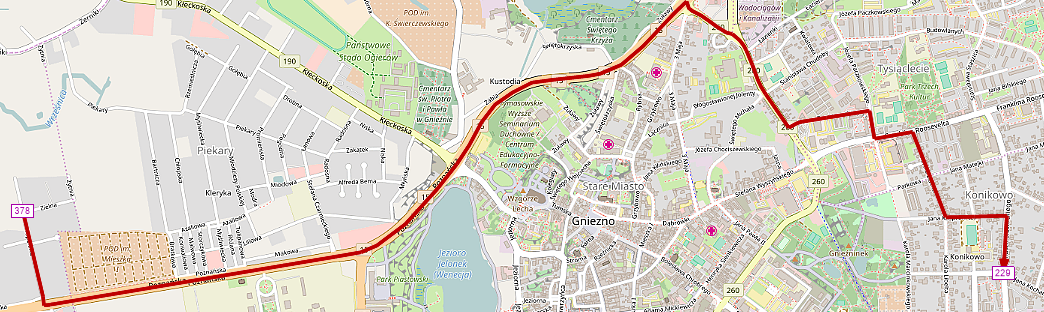
\includegraphics[height=3cm]{PGN}
\end{center}
\begin{itemize}
\male
\item sekwencja odcinków:\\
\begin{equation*}
k=\lbrace a_1, a_2,  \dots , a_n \rbrace
\end{equation*}
\item sekwencja relacji skrętnych:\\
\begin{equation*}
k=\lbrace t_1, t_2, \dots , t_n\rbrace
\end{equation*}
\item potok na ścieżce $q_k$ [poj./h]
\end{itemize}
\end{frame}

\begin{frame}{Popyt}{pojazdy podążające po ścieżkach}
\begin{center}
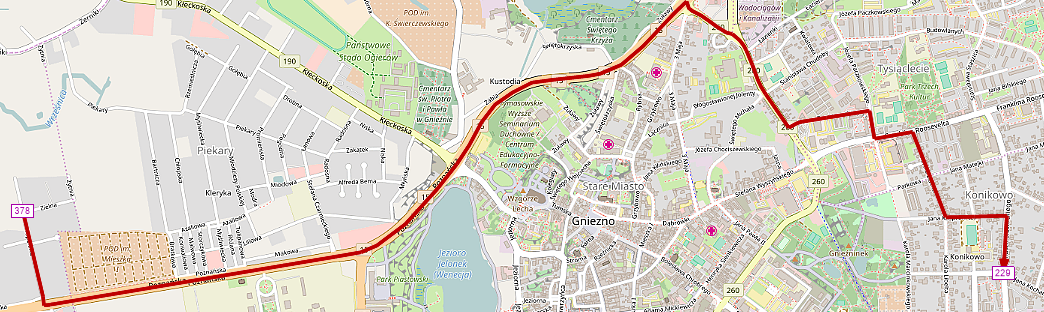
\includegraphics[height=3cm]{PGN}
\end{center}
Związek z modelem makroskpowym:
\\~\\~\\
Popyt w więźbie $q_{od}$ przemnożony p-wo wyboru ścieżki $p_{od}^k$
\begin{equation*}
q_k=q_{od}\cdot p_{od}^k
\end{equation*}
\end{frame}

\begin{frame}{Popyt}{generacja pojazdów}
Zadajemy całkowitą liczbę pojazdów $q$ na ścieżce $q_k$, albo na wlocie $q_a$. Zazwyczaj w pojazdach na godzinę.
\\Na tej podstawie generowany jest proces dopływu pojazdów:
\begin{equation*}
q_k \rightarrow \lbrace t_1, t_2, \dots , t_{q_k} \rbrace 
\end{equation*}
Gdzie odstępy $t_n - t_{n-1}$ są
\begin{itemize}
 \item stałe (model deterministyczny)
 \item zmienne (model stochastyczny)
 \end{itemize} 
\end{frame}

\begin{frame}{Popyt}{stochastyczna generacja pojazdów}
Odstępy $\Delta t = t_n - t_{n-1}$ są zazwyczaj losowane z rozkładu Poissona
\begin{equation*}
p( \Delta t ) = \frac{ {\lambda}^{\Delta t} e ^{- \lambda}}{\Delta t!}
\end{equation*}
\begin{center}
\includegraphics[height=4cm]{Poisson}
\end{center}
\male zazwyczaj generowane jest tyle samo pojazdów co zadano $\sum_{\Delta t \in q_k} p(\Delta t) = q_k$ ale trzeba pamiętać, że liczba generowanych pojazdów też jest zmienną losową.
\end{frame}

\begin{frame}{Popyt}{przypis do ścieżek}
\begin{center}
\includegraphics[height=6cm]{VissimPaths}
\end{center}
\textit{VehicleInput$\rightarrow$Volume; VehRoutDec(VehicleInput) $\rightarrow$ RelFlow}
\end{frame}

\begin{frame}{Popyt}{Granice modelu}

Pojazdy dopływają do modelu zgodnie z rozkładem Poisson'a, co jest rzadko zgodne z rzeczywistością. Zazwyczaj: \\
\male
\begin{itemize}
\item w ruchu zamiejskim jednopasowym tworzą się kolumny (\textit{platoon}) pojazdy szybsze dojeżdżają do wolniejszych
\item w ruchu zamiejskim wielopasowym zatłoczonym kolumny segregują się, mogą tworzyć sie \textit{stop-ad-go waves}, kolumny powstałe po wyprzedzających ciężarówkach itp.
\item w ruchu miejskim sterowanym pojazdy zatrzymują się przed sygnalizatorem tworzą kolumnę i ruszają z natężeniem nasycenia w rozpraszających się kolumnach.
\end{itemize}
\normalne
Dopływ Poisson'owski można stosować bezpośrednio na granicy obszaru tylko dla:
\male
\begin{itemize}
\item ruchu zamiejskiego o niewielkim zatłoczeniu (prędkość swobodna)
\item ruchu miejskiego niesterowanego o niewielkim zatłoczeniu (prędkość swobodna)
\end{itemize}
\end{frame}

\begin{frame}{Popyt}{Granice modelu}
\begin{center}
\includegraphics[height=3.5cm]{Grid}
\end{center}
W każdym innym przypadku dopływ Poissonowski można stosować na granicy poszerzonego modelu. Dopływ swobodny zostanie \textit{przefiltrowany} przez  skrzyżowania graniczne i do obszaru wpłynie już potok o innym rozkładzie (w kolumnach). 
\\ \male  \alert{rule of thumb:} dwa skrzyżowania przed wjazdem do obszaru powinny wystarczająco przefiltrować dopływ poissonowski 
\end{frame}

\subsection{Podsumowanie}
\begin{frame}{Dziękuję za uwagę}{zapraszam do dyskusji}
\bmale źródła wszystkich obrazów (jeśli nie podano inaczej) \\ M. Treiber, A. Kesting Traffic Flow Dynamics, Spirnger 2013, lub własne
\end{frame}



\end{document}
